%% ------------------------------------------------------------------------- %%
\chapter{Modelagem}
\label{cap:modelagem}

Utilizando-se da base de dados para modelagem descrita na seção "Criação da base para modelagem" (\ref{sec:criacao_da_base_para_modelagem}) - cujas variáveis explicativas foram descritas na seção "Variáveis Explicativas" (\ref{sec:variaveis_explicativas}) e a variável resposta descrita na seção "Variável Resposta" (\ref{sec:variavel_resposta}) - foram aplicados modelos de aprendizado de máquina com o intuito de obter o melhor desempenho para predição da variável resposta utilizando as variáveis explicativas construídas.

Os métodos de aprendizado de máquina utilizados foram a Regressão Linear, o Random Forest e o XGBoost, sendo que a afinação dos parâmetros de tais modelos foi feita utilizando-se o método Randomized Search. A avaliação de desempenho destes modelos foi feita utilizando-se de duas métricas, a raiz do erro quadrático médio e as bandas de acerto, e a interpretação dos modelos Random Forest e XGBoost foram feitas por meio do método Shapley Value.

\section{Análise Descritiva}
\label{sec:analise_descritiva}

A análise descritiva consiste em explorar dados utilizados para a modelagem com o intuito de encontrar a existência, ou não, de uma relação causal entre as variáveis explicativas e a variável resposta. Neste trabalho já foram apresentadas algumas análises descritivas no capítulo \ref{cap:contexto}, como, por exemplo, as estatísticas dos percentuais de polaridade obtidos da variável resposta.

Foram utilizadas 52 variáveis explicativas neste trabalho, assim, foi realizado uma verificação em cada uma das variáveis utilizando-se gráficos de dispersão. Nestes gráficos de dispersão, os valores observados para a variável explicativa estão dispostos no eixo das ordenadas e os valores observados para a variável resposta estão dispostos no eixo das abscissas. Como exemplo, abaixo está o gráfico de dispersão da variável \verb|'family_var_01_inappropriate_pct'| (que se trata do percentual de domicílios particulares permanentes em situação inadequada por município em 2000 dividido pela mesma informação em 2010), nota-se uma relação linear positiva média entre a variável explicativa e a variável resposta. Os gráficos de dispersão de todas as variáveis explicativas se encontram no anexo \ref{ape:cap3_scatter_plot}.

\graphicspath{ {./figuras/two_by_two_scatter_plot/} }
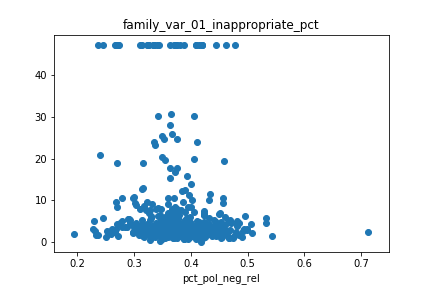
\includegraphics{04_family_var_01_inappropriate_pct}

O código citado no parágrafo anterior foi escrito na linguagem de programação Python utilizando a ferramenta Notebook Jupyter e se encontra no anexo \ref{ape:model_visualization}.

\section{Randomized Search}
\label{sec:randomized_search}

O Randomized Search é um método utilizado para otimização de hiperparâmetros que consiste em uma pesquisa aleatória sobre os hiperparâmetros fornecidos para treinamento de modelos de aprendizado de máquina visando o melhor desempenho de tal modelo. Neste trabalho foi escolhido utilizar-se o Randomized Search frente aos dois métodos mais utilizados na atualidade - o Grid Search (uma pesquisa exaustiva por meio de um subconjunto especificado manualmente do espaço de hiperparâmetros de um algoritmo de aprendizado) e a busca manual - uma vez que o Randomized Search realiza buscas mais eficientes que o Grid Search e a busca manual (ver \citet{Bergstra2012}).

Foi-se utilizada a implementação deste método proveniente da biblioteca em Python Scikit-learn (\citet{Sklearn}). Ao contrário do Grid Search, nem todos os valores dos parâmetros são testados, mas um número fixo de configurações de parâmetros é amostrado das distribuições especificadas. O número de configurações de parâmetros que são tentadas é definido pela quantidade de iterações passadas ao método e o desempenho do modelo de aprendizado de máquina treinado após a escolha dos hiperparâmetros é calculado utilizando-se do método de validação cruzada.

Se todos os parâmetros forem apresentados como uma lista, é realizada a amostragem sem reposição. Se pelo menos um parâmetro for fornecido como distribuição, é utilizada a amostragem com reposição. No âmbito deste trabalho, alguns parâmetros foram fornecidos como lista e outros como distribuição, assim, para o treinamento do modelo de aprendizado de máquina Random Forest foi-se utilizado uma amostragem com reposição e para o treinamento do modelo de aprendizado de máquina XGBoost foi-se utilizado uma amostragem sem reposição.

Além do Randomized Search ser a melhor opção por sua eficiência, existe a motivação da viabilidade da otimização dos hiperparâmetros, uma vez que para o treinamento do modelo de aprendizado de máquina XGBoost foi-se utilizado dez diferentes hiperparâmetros com diferentes quantidades de valores, representando no final uma quantidade de 1.411.200 possibilidades de cenários distintos para o treinamento.

\section{Shapley Value}
\label{sec:shapley_value}

O Shapley Value é um conceito de solução na teoria dos jogos cooperativos, foi nomeado em homenagem a Lloyd Shapley que o definiu inicialmente (ver \citet{Shapley1953}).

Em um cenário de jogos cooperativos onde, para cada jogo cooperativo, atribui-se uma distribuição única (entre os jogadores) de um excedente total gerado pelo grupo de todos os jogadores, o Shapley Value é caracterizado como uma coleção de propriedades para explicação da proveniência de cada parte desse excedente total.

A configuração é da seguinte forma: um grupo de jogadores coopera e obtém um certo ganho geral com essa cooperação. Como alguns jogadores podem contribuir mais para o grupo do que outros, ou podem ter um poder de barganha diferente, qual a importância de cada jogador para a cooperação geral e que recompensa ele pode razoavelmente esperar? Esta pergunta é uma das motivações para criação do Shapley Value, i.e., explicar essa importância individual e a recompensa esperada.

O paralelo da explicação acima à explicação do algoritmo em aprendizado de máquina seria de que os jogadores são as variáveis explicativas, o ganho geral obtido por cada jogador é o impacto na predição do modelo e a importância individual seria a importância da variável explicativa no modelo. A importância das variáveis explicativas em modelos de aprendizado de máquina é uma informação amplamente discutida, uma vez que existem diferentes formas de serem calculadas, sendo que a ordenação da importância das variáveis podem ser diferentes de um método para outro gerando discussão sobre a escolha do melhor método a ser utilizado.

O Shapley Value vem sendo considerado uma das formas mais robustas e consistentes de se avaliar a importância das variáveis explicativas (ver \citet{Lundberg2017}), ele será utilizado neste trabalho tanto para ordenação da importância das variáveis quanto para interpretação das variáveis explicativas utilizadas no modelo. Foi-se utilizada a implementação deste método proveniente da biblioteca em Python SHAP (\citet{Shap}).

\section{Métricas para avaliação de desempenho}
\label{sec:metricas_avaliacao}

Neste trabalho serão utilizadas duas métricas para avaliação de desempenho, a raiz do erro quadrático médio e a banda de acerto.

A raiz do erro quadrático médio (do inglês root mean squared error, RMSE) é uma medida frequentemente usada das diferenças entre os valores previstos por um modelo ou estimador e os valores observados. O RMSE representa a raiz quadrada da média quadrática das diferenças entre os valores previstos e os valores observados. Esses desvios são chamados de resíduos quando os cálculos são realizados sobre a amostra de dados usada para estimativa e são chamados de erros (ou erros de previsão) quando calculados fora da amostra. O RMSE é uma medida de precisão, para comparar erros de previsão de diferentes modelos para um conjunto de dados específico e não entre conjuntos de dados, pois depende da escala.

O RMSE é sempre não negativo e um valor 0 (quase nunca alcançado na prática) indicaria um ajuste perfeito para os dados. Em geral, um RMSE mais baixo é melhor que um mais alto. No entanto, comparações entre diferentes tipos de dados seriam inválidas porque a medida depende da escala dos números usados, neste trabalho, as medidas de RMSE são comparáveis uma vez que os dados trabalhados são os mesmos mudando apenas os modelos.

\begin{equation}
\mathbf {RMSE} ={\sqrt {\frac {\sum _{t=1}^{N}({\hat {y}}_{t}-y_{t})^{2}}{N}}}
\end{equation}

Sendo que,

\begin{itemize}
    \item $ \hat y_t $ representa o valor predito do modelo
    \item $ y_t $ representa o valor observado
    \item $ N $ representa a quantidade de observações
\end{itemize}

A banda de acerto é uma medida para avaliar a distribuição dos erros de predição separando-os em três categorias interpretáveis. De acordo com o valor de predição do modelo, se classifica tal predição em cada banda (tais bandas são catalogadas como "subestimado", "bem estimado" e "superestimado"). As regras para classificação em cada uma dessas opções estão listadas abaixo. O valor de $ \delta $ foi determinado empiricamente após sucessivos testes como sendo 0.15.

\begin{itemize}
	\item Subestimado: Se o valor da predição for menor que o valor observado vezes (1 - $ \delta $)
	\item Superestimado: Se o valor da predição for maior que o valor observado vezes (1 + $ \delta $)
	\item Bem estimado: Se o valor da predição estiver entre o valor observado vezes (1 - $ \delta $) e o valor observado vezes (1 + $ \delta $)
\end{itemize}

\section{Regressão Linear}
\label{sec:regressao_linear}

A regressão linear é uma abordagem para modelar a relação entre uma variável resposta (ou variável dependente) contínua e uma ou mais variáveis ​​explicativas (ou variáveis ​​independentes). É chamado de regressão linear simples quando se usa apenas uma variável explicativa, e regressão linear múltipla quando se usa mais de uma variável explicativa. Neste trabalho utilizaremos a regressão linear múltipla.

Os relacionamentos são modelados usando funções preditivas lineares cujos parâmetros desconhecidos do modelo são estimados a partir dos dados. Mais comumente, assume-se que a média condicional da resposta, dados os valores das variáveis ​​explicativas (ou preditores), seja uma função afim desses valores (função afim também é conhecida como transformação linear ($ Ax $) seguida por uma translação ($ +b $)). Como todas as formas de análise de regressão, a regressão linear se concentra na distribuição de probabilidade condicional da resposta, dados os valores dos preditores, e não na distribuição de probabilidade conjunta de todas essas variáveis.

A regressão linear foi o primeiro tipo de análise de regressão a ser estudada rigorosamente e usada extensivamente em aplicações práticas. Isso ocorre porque os modelos que dependem linearmente de seus parâmetros desconhecidos são mais fáceis de ajustar do que os modelos não linearmente relacionados aos seus parâmetros, e porque as propriedades estatísticas dos estimadores resultantes são mais fáceis de se determinar.

A regressão linear tem muitos usos práticos, o utilizado neste trabalho é o de previsão. A regressão linear pode ser usada para ajustar um modelo preditivo a um conjunto de dados observado de valores da resposta e variáveis ​​explicativas. Depois de desenvolver esse modelo, se valores adicionais das variáveis ​​explicativas forem coletados sem um valor de resposta definido, o modelo ajustado pode ser usado para fazer uma previsão da resposta.

Os modelos de regressão linear geralmente são ajustados usando a abordagem de mínimos quadrados, mas também podem ser ajustados de outras maneiras como minimizando uma versão penalizada da função custo de mínimos quadrados como na regressão de Ridge (penalidade de norma L2) e LASSO (penalidade de norma L1), mais informações de como funcionam tais técnicas de penalidade ver \citet{SantosaAndSymes1986} e \citet{Tibshirani1996}.

Dado um conjunto de dados $ {\displaystyle \{y_{i},\,x_{i1},\ldots ,x_{ip}\}_{i=1}^{n}} $ de dimensão n, um modelo de regressão linear pressupõe que a relação entre a variável dependente $ y $ e o vetor de regressores $ x $ é linear. Essa relação é modelada através de uma variável de erro $ \varepsilon $ - uma variável aleatória não observada que adiciona "ruído" à relação linear entre a variável dependente e os regressores. Assim, o modelo assume a forma:

\begin{equation}
{\displaystyle y_{i}=\beta _{0}+\beta _{1}x_{i1}+\cdots +\beta _{p}x_{ip}+\varepsilon _{i}=\mathbf {x} _{i}^{\mathsf {T}}{\boldsymbol {\beta }}+\varepsilon _{i},\qquad i=1,\ldots ,n,}
\end{equation}

onde T denota a transposição, de modo que $ {x}_{i}^{\mathsf {T}}{\boldsymbol {\beta }} $ é o produto interno entre os vetores $ {x}_{i} $ e $ \beta $.

Essas equações também podem ser representadas na notação matricial, como

\begin{equation}
{\displaystyle \mathbf {y} =X{\boldsymbol {\beta }}+{\boldsymbol {\varepsilon }},\,}
\end{equation}

onde

\mathbf {y} ={\begin{pmatrix}y_{1}\\y_{2}\\\vdots \\y_{n}\end{pmatrix}}, X={\begin{pmatrix}\mathbf {x} _{1}^{\mathsf {T}}\\\mathbf {x} _{2}^{\mathsf {T}}\\\vdots \\\mathbf {x} _{n}^{\mathsf {T}}\end{pmatrix}}={\begin{pmatrix}1&x_{11}&\cdots &x_{1p}\\1&x_{21}&\cdots &x_{2p}\\\vdots &\vdots &\ddots &\vdots \\1&x_{n1}&\cdots &x_{np}\end{pmatrix}}, {\boldsymbol {\beta }}={\begin{pmatrix}\beta _{0}\\\beta _{1}\\\beta _{2}\\\vdots \\\beta _{p}\end{pmatrix}, {\boldsymbol {\varepsilon }}={\begin{pmatrix}\varepsilon _{1}\\\varepsilon _{2}\\\vdots \\\varepsilon _{n}\end{pmatrix}}.}

Sendo que as terminologias são:

\begin{itemize}
	\item $ \mathbf {y} $ é um vetor de valores observados $ y_{i} (i = 1, \ldots, n) $ também conhecido como variável resposta ou variável dependente. Essa variável não deve ser confundida com os valores previstos, que são indicados como $ \hat{y} $. A decisão sobre qual variável em um conjunto de dados ser modelada como variável dependente e quais são modeladas como variáveis ​​independentes baseia-se na presunção de que o valor de uma das variáveis ​​é causado por, ou diretamente influenciado por outras variáveis.

	\item $ X $ pode ser visto como uma matriz de vetores de linha $ \mathbf {x}_{i} $, conhecidos como variáveis ​​explicativas ou variáveis ​​independentes. Geralmente, uma constante é incluída como um dos regressores, o elemento correspondente de $ \beta $ é chamado de intercepto. Muitos procedimentos de inferência estatística para modelos lineares exigem a presença de um intercepto, por isso o mesmo é frequentemente incluído, mesmo que considerações teóricas sugiram que seu valor seja zero.

	\item $ \beta $ é um vetor de parâmetro dimensional $ (p + 1) $, em que $ \beta_{0} $ é o termo de intercepto (se houver um no modelo - caso contrário, $ \beta $ é p-dimensional). Seus elementos são conhecidos como efeitos ou coeficientes de regressão, embora o último termo as vezes seja reservado para os efeitos estimados. A estimativa estatística e inferência na regressão linear se concentra em $ \beta $, os elementos desse vetor de parâmetro são interpretados como derivadas parciais da variável dependente em relação às várias variáveis ​​independentes.

	\item $ \varepsilon $ é um vetor de valores $ \varepsilon_{i} $. Essa parte do modelo é chamada de termo de erro ou, as vezes, ruído. Essa variável captura todos os outros fatores que influenciam a variável dependente $ y $, exceto os regressores $ x $. A relação entre o termo de erro e os regressores, por exemplo, sua correlação, é uma consideração crucial na formulação de um modelo de regressão linear, pois determinará o método de estimativa apropriado.
\end{itemize}

Uma explicação mais detalhada sobre como a regressão linear estima seus parâmetros pode ser encontrada em \citet{Freedman2009}.

Neste trabalho, o treinamento da regressão linear foi feito utilizando-se a biblioteca em Python scikit-learn (\citet{Sklearn}) que é uma das bibliotecas mais utilizadas para treinamento de modelos de aprendizado de máquina na linguagem de programação Python.

O modelo de regressão linear é relativamente simples e de fácil interpretabilidade, uma boa estratégia de modelagem é no início do processo de modelagem realizar o treinamento do mesmo e utilizar seu desempenho como base para comparação futura com outros experimentos utilizando-se de outros modelos de aprendizado de máquina. Assim, tal modelo foi utilizado apenas para obter um desempenho base.

As estimativas para os parâmetros deste modelo podem ser encontradas no apêndice \ref{tab:cap3_estimativa_reg_lin}. Em alguns casos nota-se que houve inversão de estimativas com relação ao esperado, como exemplo de tal inversão temos os gráficos de dispersão das variáveis explicativas \verb|"enem_var_01_enem_score_mean_pct"| e \verb|"enem_var_01_enem_score_median_pct"| (presentes no apêndice \ref{ape:cap3_scatter_plot}). Tais gráficos mostram uma dispersão de valores muito próxima entre as duas variáveis, conceitualmente também é esperado que a relação com a variável resposta seja semelhante, porém as estimativas são estritamente opostas assumindo os valores 0.33489 e -0.34682, respectivamente.

O desempenho do modelo será avaliado, conforme mencionado anteriormente, utilizando-se as medidas RMSE e bandas de acerto. Na tabela \ref{tab:cap3_rmse_reg_lin} apresenta-se o RMSE sobre a base de treinamento ("Treino"), sobre a base de validação ("Validação") e o RMSE calculado sobre a base de validação utilizando-se um modelo aleatório ("Validação (modelo aleatório)"). O modelo aleatório apresenta um número aleatório que esteja entre o mínimo e o máximo observado na validação, foi criado apenas para critério de comparação com o modelo de regressão linear. Nota-se um erro estritamente superior do modelo aleatório sobre o erro da regressão linear, o que implica na possibilidade da previsão da variável resposta utilizando-se das variáveis explicativas existentes.

Na tabela \ref{tab:cap3_band_reg_lin} apresenta-se a banda de acerto sobre a base de treinamento ("Treino"), sobre a base de validação ("Validação") e a banda de acerto calculada sobre a base de validação utilizando-se um modelo aleatório ("Validação (modelo aleatório)"). Nota-se que a regressão linear teve a maior concentração em "Bem Estimado" com quase 70\% na validação, e 80\% no treino.

No gráfico \ref{ape:cap3_scatter_reg_lin} nota-se, apesar de suave, uma relação de linearidade entre os valores preditos (eixo das ordenadas) e os valores observados (eixo das abscissas) em ambas bases de dados (treino e validação).

\section{Random Forest}
\label{sec:random_forest}

O Random Forest é um método de aprendizado de máquina para classificação e regressão que opera construindo várias árvores de decisão (classificação) ou árvores de regressão (regressão), sendo que a predição de tal método é dada pela moda dos valores preditos em cada árvore, no caso da classificação, ou é dada pela média dos valores preditos em cada árvore, no caso de regressão. A forma de seleção aleatória das árvores reduz a incidência de overfitting no treino sobre a base de treinamento.

O Random Forest foi criado por Tin Kam Ho em (ref.) usando o método do subespaço aleatório, que, na formulação de Ho, é uma maneira de implementar a abordagem de "discriminação estocástica" à classificação proposta por Eugene Kleinberg (ver ref.).

O algoritmo é primordialmente baseado em árvores de decisão que é um método popular para várias tarefas de aprendizado de máquina. A árvore de decisão atende aos requisitos para servir como um procedimento de prateleira para mineração de dados, porque é invariável à escala e transformações em variáveis explicativas, é robusto para inclusão de variáveis irrelevantes e seu resultado, na maioria das vezes, é interpretável.

Em particular, árvores muito profundas tendem a aprender padrões altamente irregulares: elas superestimam seus conjuntos de treinamento, ou seja, têm um viés baixo, mas uma variação muito alta (comumente conhecido como bias-variance tradeoff). O Random Forest é uma maneira de calcular a média de várias árvores de decisão, treinadas em diferentes partes do mesmo conjunto de treinamento, com o objetivo de reduzir a variação. Isso ocorre às custas de um pequeno aumento no viés e perda de interpretabilidade - uma vez que são criadas diversas árvores -, mas geralmente se aumenta muito o desempenho no modelo final.

O algoritmo de treinamento para o Random Forest aplica a técnica geral de agregação de bootstrap conhecido como Bagging. Dado um conjunto de treinamento $ {\displaystyle X = x_{1},\ldots ,x_{n}} $ com respostas $ {\displaystyle Y = y_{1},\ldots ,y_{n}} $, selecionados repetidamente $ B $ vezes, seleciona-se uma amostra aleatória com repetição do conjunto de treinamento e se realiza o treinamento das árvores a essas amostras:





For b = 1, ..., B:

Sample, with replacement, n training examples from X, Y; call these Xb, Yb.
Train a classification or regression tree fb on Xb, Yb.
After training, predictions for unseen samples x' can be made by averaging the predictions from all the individual regression trees on x':

{\displaystyle {\hat {f}}={\frac {1}{B}}\sum _{b=1}^{B}f_{b}(x')}

or by taking the majority vote in the case of classification trees.

This bootstrapping procedure leads to better model performance because it decreases the variance of the model, without increasing the bias. This means that while the predictions of a single tree are highly sensitive to noise in its training set, the average of many trees is not, as long as the trees are not correlated. Simply training many trees on a single training set would give strongly correlated trees (or even the same tree many times, if the training algorithm is deterministic); bootstrap sampling is a way of de-correlating the trees by showing them different training sets.

The above procedure describes the original bagging algorithm for trees. Random forests differ in only one way from this general scheme: they use a modified tree learning algorithm that selects, at each candidate split in the learning process, a random subset of the features. This process is sometimes called "feature bagging". The reason for doing this is the correlation of the trees in an ordinary bootstrap sample: if one or a few features are very strong predictors for the response variable (target output), these features will be selected in many of the B trees, causing them to become correlated. An analysis of how bagging and random subspace projection contribute to accuracy gains under different conditions is given by Ho.[14]

Typically, for a classification problem with p features, √p (rounded down) features are used in each split.[3]:592 For regression problems the inventors recommend p/3 (rounded down) with a minimum node size of 5 as the default.[3]:592. In practice the best values for these parameters will depend on the problem, and they should be treated as tuning parameters[3]:592.































\section{XGBoost}
\label{sec:xgboost}

(?).

%% ------------------------------------------------------------------------- %%